\chapter[Proposta]{Proposta}
\label{chap:Proposta}
Neste capítulo, é retomado o contexto em que o trabalho pretende contribuir, apresentando a proposta do Trabalho de Conclusão de Curso. Inicialmente, na seção \hyperref[sec:Contextualizacao]{Contextualização} (Seção \hyperref[sec:Contextualizacao]{5.1}), é 
apresentado o domínio em que o estudo está inserido. Adicionalmente, com intuito de apresentar adequadamente a aplicação, a seção \hyperref[sec:Detalhamento da Aplicacao]{Detalhamento da Aplicação} (Seção \hyperref[sec:Detalhamento da Aplicacao]{5.2}) é exposta. 
Com base nos insumos obtidos no primeiro ciclo de teste, a seção \hyperref[sec:Melhorias Propostas]{Melhorias Propostas} (Seção \hyperref[sec:Melhorias Propostas]{5.3}) elucida sobre a incorporação das melhorias elicitadas junto ao público 
alvo no aplicativo em estudo, o que demandou refinamentos no protótipo de alta fidelidade, em especial no fluxo de \hyperref[sec:Onboarding]{\textit{Onboarding}}, e na disposição de informações em geral. Com base nesses resultados, a \hyperref[sec:Matriz SWOT]{Matriz SWOT} (Seção \hyperref[sec:Matriz SWOT]{5.4}) apresenta as forças, fraquezas, 
ameaças e oportunidades identificadas durante a análise da versão evoluída do aplicativo. Ademais, encontra-se a \hyperref[sec:Backlog de Melhorias]{\textit{Backlog} de Melhorias priorizado} (Seção \hyperref[sec:Backlog de Melhorias]{5.5}), no qual constam as principais funcionalidades que serão implementadas 
de fato no aplicativo, com base no protótipo de alta fidelidade validado em dois ciclos de teste. Por fim, tem-se o \hyperref[sec:Resumo Proposta]{Resumo do Capítulo} (Seção \hyperref[sec:Resumo Proposta]{5.9}).

\section{Contextualização}
\label{sec:Contextualizacao}
O presente trabalho tem como objetivo principal investigar as melhorias na usabilidade e na experiência do usuário de um aplicativo móvel chamado Multilind, desenvolvido para o mapeamento das línguas indígenas do Brasil. 
De acordo com \citeonline{bevan1995}, usabilidade é o termo técnico usado para descrever a qualidade de uso de uma interface. Em outras palavras, refere-se à facilidade com que os usuários podem interagir e realizar 
tarefas em um sistema, aplicativo ou site. Uma interface com boa usabilidade é aquela que proporciona uma experiência fluida, intuitiva e eficiente para os usuários. Complementarmente, a experiência de usuário preocupa-se 
com as percepções e respostas do usuário antes, durante e após o uso da aplicação \cite{iso9241210}.

O Multilind foi desenvolvido em parceria com a professora Altaci Corrêa Rubim\footnote{\url{https://amazoniareal.com.br/personagem/altaci-correa-rubim/}(último acesso: Março 2024)}, representante brasileira do Grupo de Trabalho Mundial da Década das Línguas Indígenas, 
e membros do GT do Brasil. O aplicativo foi criado durante disciplinas de Métodos de Desenvolvimento de Software e Engenharia de Produto de Software da Universidade de Brasília - Campus Gama, utilizando a licença MIT. Ele possui funcionalidades que permitem o mapeamento 
das línguas indígenas, fornecendo informações sobre cada língua, como família linguística, área de ocorrência, palavras e suas traduções.

Considerando que é uma aplicação já existente, para implementar tais melhorias, foram consideradas as heurísticas de Nielsen, que são diretrizes elaboradas para garantir que as interfaces do sistema atendam aos princípios fundamentais de usabilidade. Além disso, em um 
primeiro momento, para maior familiaridade da autora às demandas, propõe-se o uso de provas de conceitos, orientadas a ciclos de teste de usabilidade. 

Adiante, com o avançar do trabalho na segunda etapa do TCC, pretende-se seguir de forma mais rigorosa as etapas de 
pesquisa-ação, estabelecidas para condução da análise de resultados do trabalho com um todo. O foco das provas de conceito é o atendimento adequado das necessidades e expectativas, tanto dos usuários do aplicativo Multilind, quanto da equipe envolvida. A ideia é tratar 
demandas mais prioritárias, e não a completude das demandas. Essa decisão foi tomada considerando prazos e desenvolvimento solo da autora.

Na primeira etapa do TCC, foram desenvolvidos protótipos que permitiram a visualização e a avaliação preliminar das melhorias propostas em termos de usabilidade e experiência do usuário. Os protótipos 
foram submetidos a avaliações junto ao público alvo, permitindo, desde o começo do trabalho, ajustes e refinamentos com base no \textit{feedback} obtido. 

Uma vez cumprida com essa etapa inicial de validação dos protótipos, a segunda etapa do trabalho consistirá no desenvolvimento efetivo do aplicativo Multilind evoluído, orientando-se pelas melhorias identificadas. 

Com base nas lições aprendidas durante a fase de prototipação, funcionalidades serão implementadas, além da realização de testes mais aprofundados, a fim de garantir que a interface final do aplicativo atenda aos critérios de usabilidade e proporcione uma maior satisfação, engajamento e facilidade de uso. No intuito de conferir uma visão 
mais concreta sobre o objeto de estudo deste trabalho, segue o \hyperref[sec:Detalhamento da Aplicacao]{Detalhamento da Aplicação}.
	
\section{Detalhamento da Aplicação}
\label{sec:Detalhamento da Aplicacao}
Ressalta-se a relevância de explorar em detalhes o aplicativo Multilind, em sua versão v.1.4.0. Como a aplicação já se encontra desenvolvida, em sua primeira versão, há necessidade de conhecer e revelar sobre Arquitetura, Público-Alvo, Guia de Estilo e Funcionalidades. Esses aspectos são 
tratados na sequência. O compromisso da autora é não violar o entorno do aplicativo Multilind, sejam as expectativas dos usuários que já consomem o aplicativo, e reconhecem no mesmo funcionalidades bem ajustadas; sejam as noções técnicas, com uso de tecnologias já estabelecidas.

\subsection{Arquitetura}
\label{Arquitetura}
O projeto do aplicativo Multilind contém três repositórios principais: o respositório de \textit{Frontend}, que armazena a camada que lida com as interfaces do usuário, desenvolvido em React Native; o repositório \textit{Content Server}, que armazena os conteúdos do sistema 
utilizando PostgreSQL, e o repositório \textit{Files Server}, responsável por armazenar e administrar os arquivos de mídia do aplicativo. Os diagramas de  pacotes, correspondentes a cada repositório, podem ser conferidos nas Figuras \ref{fig08}, \ref{fig09} e \ref{fig10}. 

Na Figura \ref{fig08}, sobre o Frontend, há estruturação dos pacotes orientando-se pelo estilo arquitetural N-Camadas, com destaque aos pacotes de maior nível de abstração, ou seja, os pacotes que atuam na camada de interface com o usuário. Por isso, há destaque aos pacotes das bibliotecas, representados de forma generalista, 
como \textit{Library1} a \textit{Library N}, por não haver necessidade de revelar cada biblioteca em si; aos pacotes que representam as telas, seus contextos e serviços, e aos pacotes que compreendem os componentes, sendo esses estruturados em obediência ao conceito de Atomic Design \cite{atomic}. 

Atomic Design, em linhas bem gerais, é uma abordagem que permite estruturar os elementos de \textit{design} usando uma analogia com átomos, moléculas, organismos e \textit{templates}, conforme descrito:

\begin{itemize}
	\item Átomos - componentes arquiteturais de menor nível de granularidade. Ex. Elementos Básicos: fontes, imagens, formas, ícones e cores;
	\item Moléculas - componentes arquiteturais de segundo menor nível de granularidade. Ex. Forma (átomo) e Texto (átomo) juntos para formar um Botão (molécula);
	\item Organismos - componentes arquiteturais de terceiro menor nível de granularidade. Ex. Estruturas como menu, \textit{header}, e \textit{footers};
	\item \textit{Templates} - componentes arquiteturais de quarto menor nível de granularidade (penúltimo). Ex. Agrupando organismos, têm-se \textit{templates}, que são utilizados em protótipos e \textit{wireframes}, 
	\item Páginas - componentes arquiteturais de maior nível de granularidade. Ex. Instâncias específicas de \textit{template}.
\end{itemize}

Na Figura \ref{fig09}, sobre o \textit{Content Server}, também há estruturação dos pacotes orientando-se pelo estilo arquitetural N-Camadas, com destaque aos pacotes inerentes ao lado do servidor, considerando uma arquitetura Cliente-Servidor. Por isso, há menção aos pacotes das \textit{Controllers}, sendo essas responsáveis, em um padrão 
arquitetural MVC \textit{(Model-View-Controller)} \cite{designpattern}, por intermediar as comunicações entre a camada de Visão (no Multilind, a grosso modo, representado por \textit{Frontend}) e a camada de Modelo (no Multilind, a grosso modo, representado por \textit{Functions}). Cabe destacar ainda o pacote \textit{Services}, o qual corresponde ao banco 
de dados (no caso do Multilind, o banco de dados PostgreSQL) \cite{larman2004}.

Na Figura \ref{fig10}, sobre o \textit{Files Server}, também há estruturação dos pacotes orientando-se pelo estilo arquitetural N-Camadas. Similarmete, ao caso do servidor anterior, há destaque aos pacotes inerentes ao lado do servidor, com \textit{Controllers} e \textit{Services}. Cabe enfatizar que o aplicativo Multilind, portanto, compartilha de 
uma arquitetura híbrida, que combina vários estilos e padrões arquiteturais, tais como: N-Camadas, Cliente-Servidor e MVC.

\begin{figure}[h]
	\centering
	\caption{Diagrama de Pacotes \textit{Frontend}}
	\begin{adjustbox}{center}
		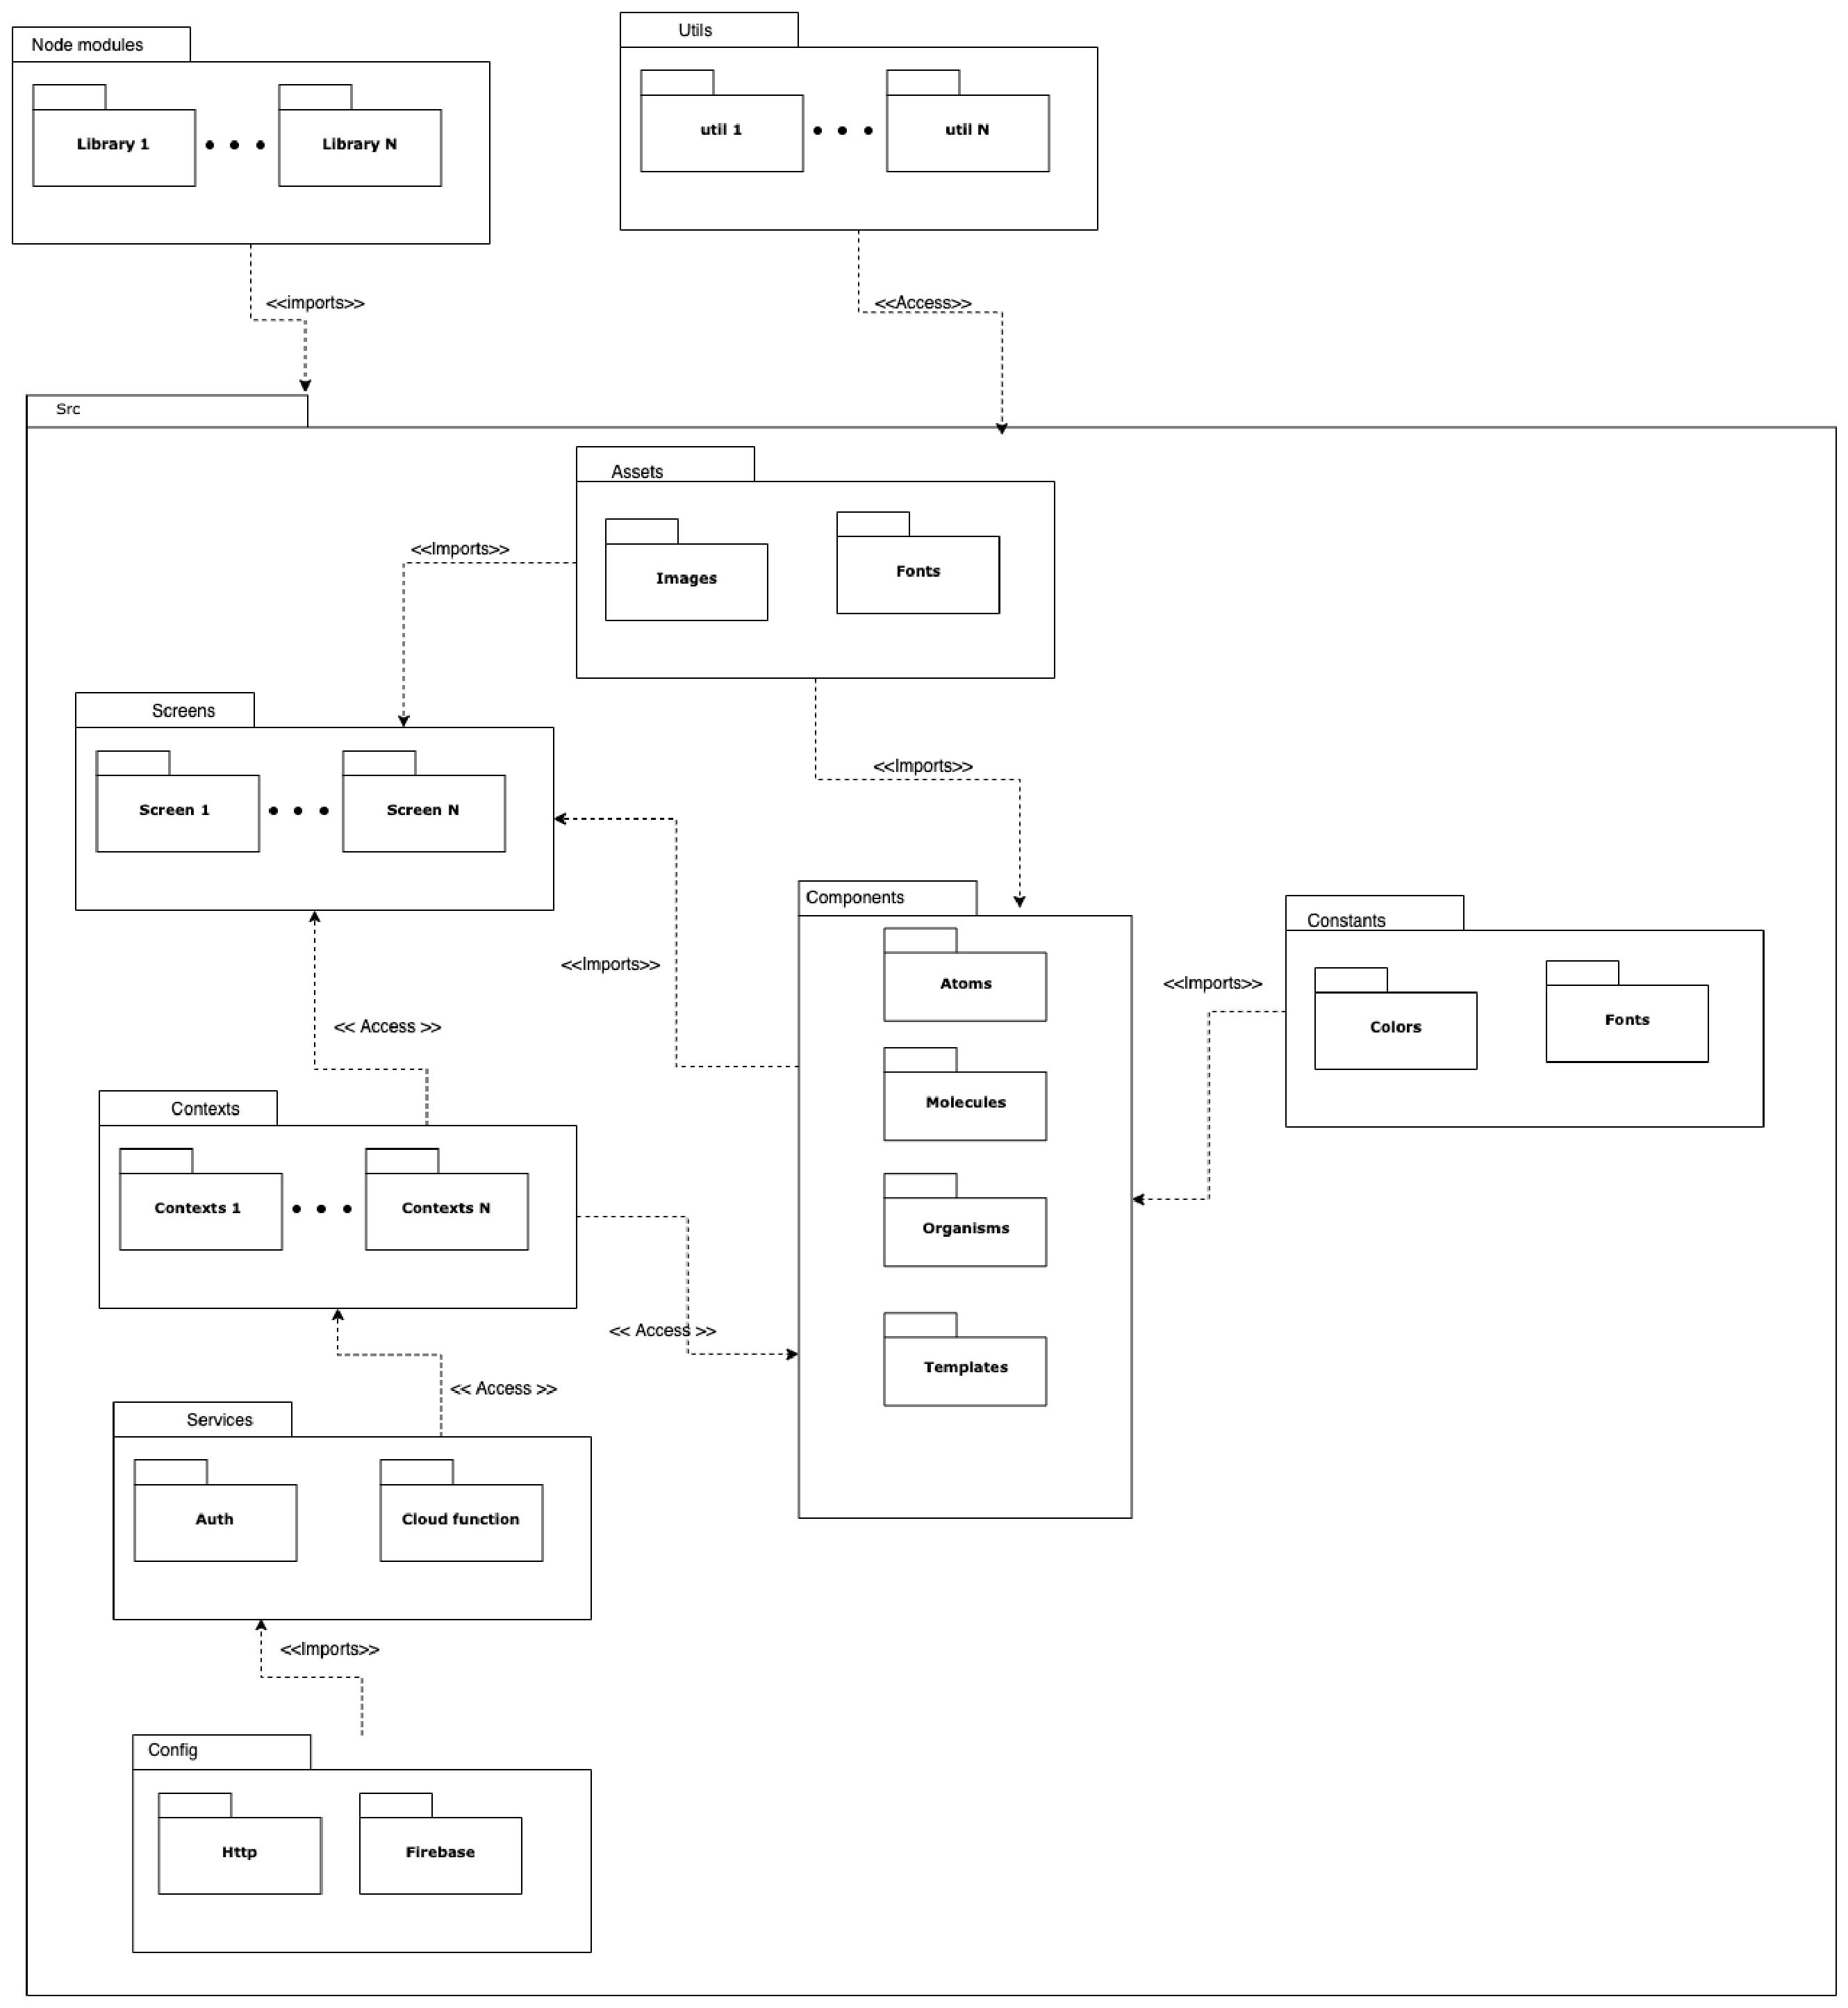
\includegraphics[width=1\textwidth]{figuras/frontend.eps}
	\end{adjustbox}
	\begin{tablenotes}[flushleft]
		\centering
		\item \textit{Fonte:} Autora.
	\end{tablenotes}
	\label{fig08}
\end{figure}

\pagebreak

\begin{figure}[h!]
	\centering
	\caption{Diagrama de Pacotes \textit{Content Server}}
	\begin{adjustbox}{center}
		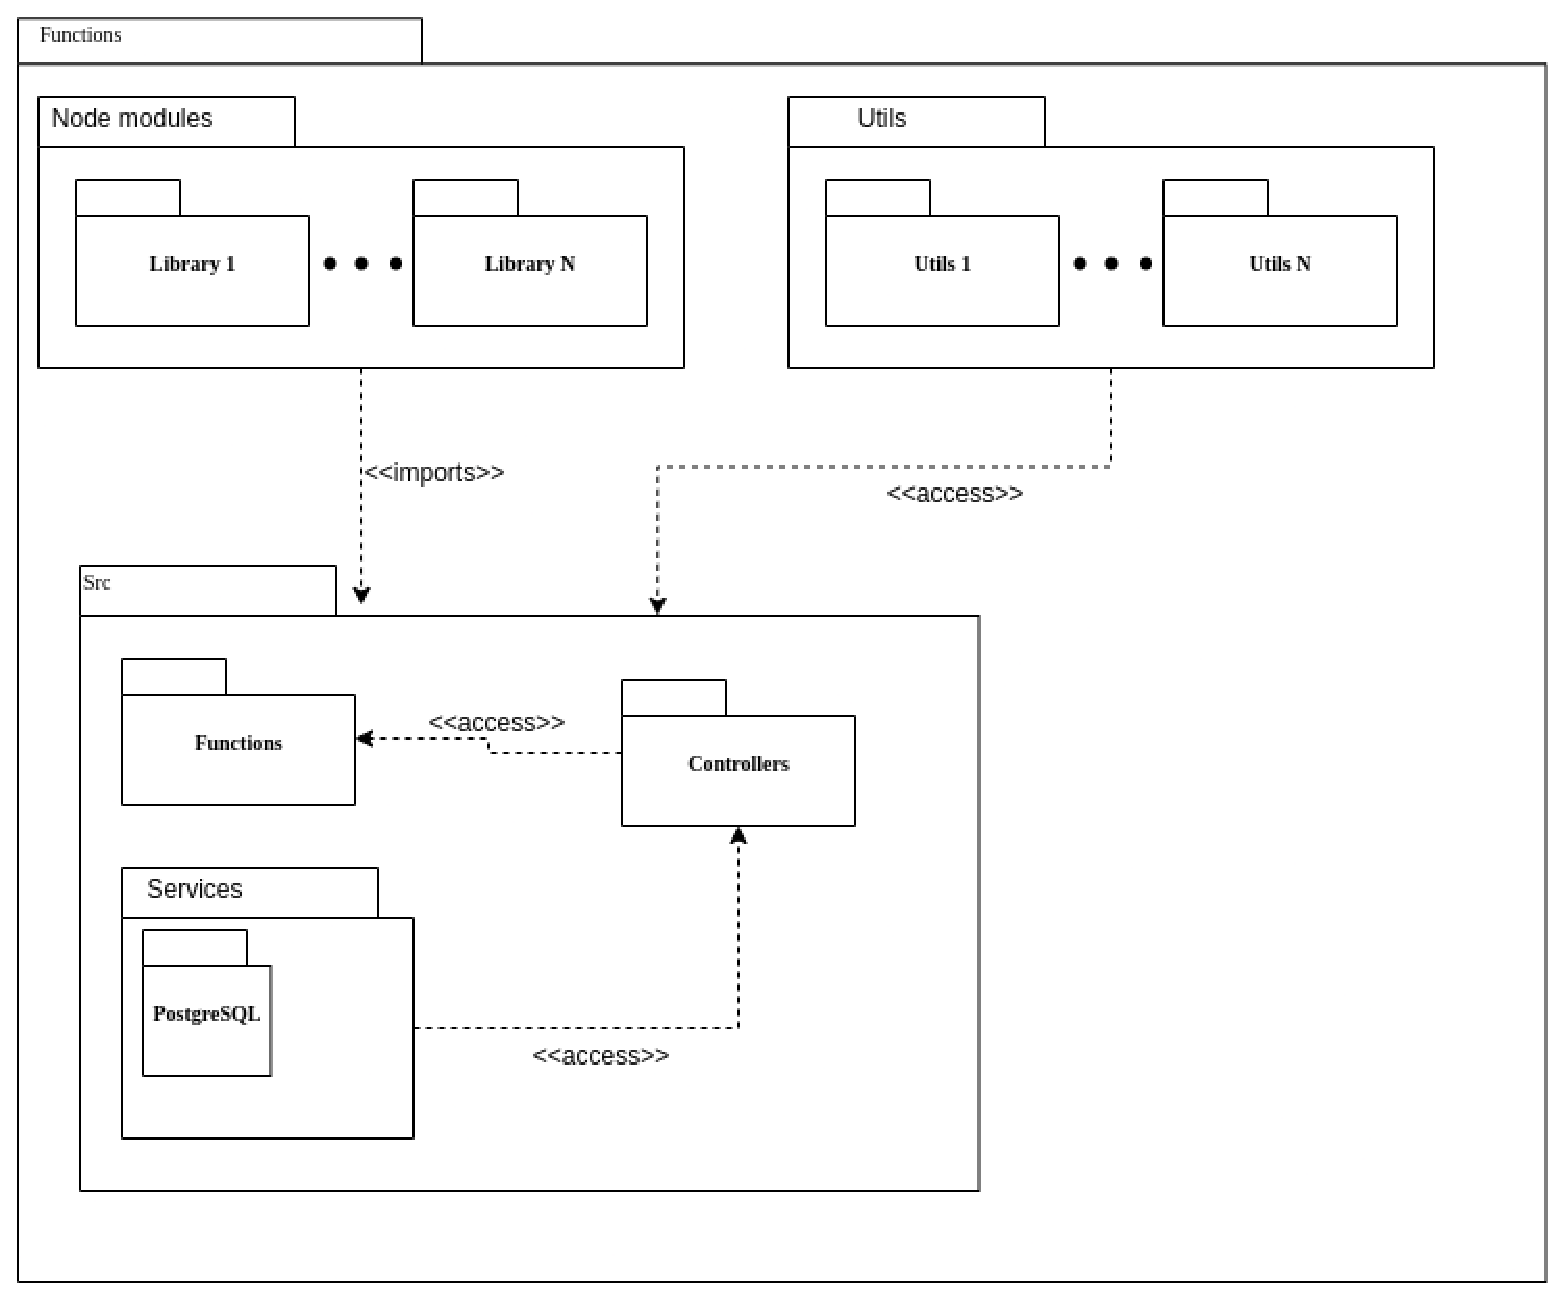
\includegraphics[width=0.8\textwidth]{figuras/content.eps}
	\end{adjustbox}
	\begin{tablenotes}[flushleft]
		\centering
		\item \textit{Fonte:} Autora.
	\end{tablenotes}
	\label{fig09}
\end{figure}

\begin{figure}[h!]
	\centering
	\caption{Diagrama de Pacotes \textit{Files Server}}
	\begin{adjustbox}{center}
		\includegraphics[width=0.8\textwidth]{figuras/files.eps}
	\end{adjustbox}
	\begin{tablenotes}[flushleft]
		\centering
		\item \textit{Fonte:} Autora.
	\end{tablenotes}
	\label{fig10}
\end{figure}

\subsection{Público-Alvo}
\label{Publico-Alvo}
A Lean Inception, criada por \citeonline{lean}, foi utilizada como forma de alinhar os desenvolvedores e \textit{stakeholders} em relação ao aplicativo, antes de sua execução, e confirmar sua viabilidade e sua necessidade. O processo aborda a visão do produto; a compreensão de personas; suas jornadas de usuário, e 
o desenvolvimento de funcionalidades de alto nível \cite{lean}. No estágio de definição da visão do produto, a equipe e os \textit{stakeholders} do projeto responderam questões relativas ao público alvo da aplicação; o objetivo, e as principais características, como pode ser visto nas 
Figuras \ref{fig11} e \ref{fig12}. 

Com base na Figura \ref{fig11}, sobre o foco do produto em povos indígenas e todos que possuem interesse sobre linguas indígenas; bem como em aspectos qualitativos, tais como: praticidade, acessibilidade, atualidade 
e disponibilidade. 

\begin{figure}[h!]
	\centering
	\caption{Visão de Produto}
	\begin{adjustbox}{center}
		\includegraphics[width=0.75\textwidth]{figuras/visao_produto.eps}
	\end{adjustbox}
	\begin{tablenotes}[flushleft]
		\centering
		\item \textit{Fonte:} Multilind.
	\end{tablenotes}
	\label{fig11}
\end{figure}
Na Figura \ref{fig12}, estrutura-se a definição do produto considerando: "É'', com destaque em é interativo, prático, mobile, gratuito, dentre outros; "NÃO É'', mencionando que não é jogo, rede social, chat, site, blog ou fórum, tampouco complexo; "FAZ'', com menção a fazer mapeamento de línguas, 
pesquisa por palavras, dentre outros; "NÃO FAZ'', destacando que não faz restrição ao acesso à informação, nem expõe dados pessoais, dentre outros.

\begin{figure}[h!]
	\centering
	\caption{Definição do Produto}
	\begin{adjustbox}{center}
		\includegraphics[width=1\textwidth]{figuras/produto_e_nao_e.eps}
	\end{adjustbox}
	\begin{tablenotes}[flushleft]
		\centering
		\item \textit{Fonte:} Multilind.
	\end{tablenotes}
	\label{fig12}
\end{figure}

Como definidas no Capítulo de \hyperref[chap:Referencial]{Referencial Teórico}, as personas são representações detalhadas de perfis semifictícios, sendo desenvolvidas para ajudar a equipe na melhor compreensão sobre os usuários, bem 
como sobre suas necessidades e expectativas. 

Ainda durante a Lean Inception, na fase de descrição de personas, foram criadas três personas que representam diferentes tipos de usuários do aplicativo. Essas personas foram essenciais para realizar as jornadas das personas, e levantar as 
funcionalidades necessárias para atender às necessidades e expectativas dos envolvidos. As Figuras \ref{fig13}, \ref{fig14} e \ref{fig15} mostram os três principais perfis levantados.  Na Figura \ref{fig13}, tem-se a persona Helena, de 24 anos, pós 
graduanda em psicologia, com interesses como Cultura Indígena; comportamentes como gostar de viajar pelo Brasil, e necessidades, como localizar povos indígenas por regiões. Na figura \ref{fig14}, encontra-se a persona Kauã, de 40 anos, indígena do povo 
Guarani, professor, que tem interesse em mostrar novas línguas indígenas a seus alunos. Por último, na Figura \ref{fig15} tem-se a persona Flávia, 45 anos, linguista, professora e pesquisadora; possui bastante conhecimento acerca de línguas indígenas e 
tem interesse em contribuir com o projeto.

\begin{figure}[h!]
	\centering
	\caption{Persona 1}
	\begin{adjustbox}{center}
		\includegraphics[width=1.7\textwidth]{figuras/persona1.eps}
	\end{adjustbox}
	\begin{tablenotes}[flushleft]
		\centering
		\item \textit{Fonte:} Autora.
	\end{tablenotes}
	\label{fig13}
\end{figure}

\begin{figure}[h!]
	\centering
	\caption{Persona 2}
	\begin{adjustbox}{center}
		\includegraphics[width=2.5\textwidth]{figuras/persona2.eps}
	\end{adjustbox}
	\begin{tablenotes}[flushleft]
		\centering
		\item \textit{Fonte:} Autora.
	\end{tablenotes}
	\label{fig14}
\end{figure}

\pagebreak

\begin{figure}[h!]
	\centering
	\caption{Persona 3}
	\begin{adjustbox}{center}
		\includegraphics[width=2.5\textwidth]{figuras/persona3.eps}
	\end{adjustbox}
	\begin{tablenotes}[flushleft]
		\centering
		\item \textit{Fonte:} Autora.
	\end{tablenotes}
	\label{fig15}
\end{figure}

\subsection{Guia de Estilo}
\label{Guia de Estilo}
O guia de estilo do produto foi desenvolvido a partir da criação de um Manual de Identidade Visual\footnote{Manual de Identidade Visual Multilind, 2021. Disponível
em: \url{https://fga-eps-mds.github.io/2021.1-Multilind-Docs/img/manualIdentidade/Manual_Id.pdf} (último acesso: Março 2024)}. Esse manual definiu os elementos fundamentais da marca, incluindo cores, tipografia, aplicação da marca, símbolo e conceitos base.

O símbolo do Multilind é representado pelo beija-flor, que simboliza a pajé e a espiritualidade da língua. As principais cores presentes na logomarca são representadas pelos hexadecimais "\#04B47F'' e "\#338BAE''. Além disso, outras cores foram selecionadas 
como base para o desenvolvimento do \textit{design} de interface da aplicação, que podem ser vistas nas Figuras \ref{fig16} e \ref{fig17}.

\begin{figure}[h!]
	\centering
	\caption{Paleta de Cores - Verde}
	\begin{adjustbox}{center}
		\includegraphics[width=0.7\textwidth]{figuras/cor1.eps}
	\end{adjustbox}
	\begin{tablenotes}[flushleft]
		\centering
		\item \textit{Fonte:} Autora.
	\end{tablenotes}
	\label{fig16}
\end{figure}

\begin{figure}[h!]
	\centering
	\caption{Paleta de Cores - Azul}
	\begin{adjustbox}{center}
		\includegraphics[width=0.7\textwidth]{figuras/cor2.eps}
	\end{adjustbox}
	\begin{tablenotes}[flushleft]
		\centering
		\item \textit{Fonte:} Autora.
	\end{tablenotes}
	\label{fig17}
\end{figure}

\subsection{Funcionalidades}
\label{Funcionalidades}
A versão 1.4.0 da aplicação possui diversas funcionalidades voltadas para o mapeamento e a divulgação das línguas indígenas brasileiras. Entre essas funcionalidades, destaca-se o mapeamento das línguas, que permite aos usuários 
explorar através do mapa e descobrir informações sobre línguas indígenas brasileiras. Isso inclui detalhes sobre o tronco e a família linguística à qual a língua pertence, seu dicionário e imagens relativas à lista de palavras.


A representação das telas do aplicativo pode ser vista nas Figuras \ref{fig18} e \ref{fig19}. Na Figura \ref{fig18}, são apresentadas as telas do mapa e palavra específica. O mapa permite visualizar a localização geográfica das 
línguas indígenas, enquanto a tela de palavra específica exibe detalhes sobre palavras específicas de cada língua. Já na Figura \ref{fig19}, são apresentadas as telas de línguas e dicionário. A tela de línguas permite explorar 
as diferentes línguas indígenas disponíveis no aplicativo, enquanto o dicionário oferece acesso a palavras e seus respectivos significados. 

Além disso, a aplicação também oferece recursos de tradução para o português indígena e o português formal. Os usuários podem fazer buscas por palavras e visualizar informações como significado e imagens relativas. Um levantamento 
mais pleno sobre essas funcionalidades pode ser obtido consultando o repositório do aplicativo Multilind. Nesse repositório, a equipe procurou destacar sobre os principais propósitos do aplicativo. \footnote{Repositório Multilind, 2023. Disponível
em: \url{https://fga-eps-mds.github.io/2021.1-Multilind-Docs/} (último acesso: Março 2024)}

\begin{figure}[h!]
	\centering
	\caption{Telas da Aplicação - Mapa e Palavra Específica}
	\begin{adjustbox}{center}
		\includegraphics[width=1\textwidth]{figuras/app1.eps}
	\end{adjustbox}
	\begin{tablenotes}[flushleft]
		\centering
		\item \textit{Fonte:} Autora.
	\end{tablenotes}
	\label{fig18}
\end{figure}

\newpage

\begin{figure}[h!]
	\centering
	\caption{Telas da Aplicação - Línguas e Dicionário}
	\begin{adjustbox}{center}
		\includegraphics[width=0.9\textwidth]{figuras/app2.eps}
	\end{adjustbox}
	\begin{tablenotes}[flushleft]
		\centering
		\item \textit{Fonte:} Autora.
	\end{tablenotes}
	\label{fig19}
\end{figure}

\section{Melhorias Propostas}
\label{sec:Melhorias Propostas}
Ao buscar realizar melhorias na aplicação e reconhecendo a importância de envolver usuários reais nas tomadas de decisões, testes de usabilidade foram feitos e \textit{feedbacks} coletados, 
o que orientou o processo de melhoria de usabilidade e experiência de usuário. Ocorreu ainda a aplicação das heurísticas de Nielsen. Os resultados constam no prótotipo, já modelado com as melhorias
\footnote{Protótipo com melhorias. Disponível em: \url{https://shorturl.at/ryEOR}(último acesso: Março 2024)}. Particularidades sobre cada melhoria constam nas próximas seções.

\subsection{\textit{Onboarding}}
\label{sec:Onboarding}
Seguindo a abordagem de \citeonline{cooper2007}, o \textit{design} depende do contexto - quem são os usuários; o que estão fazendo, e seus objetivos. Além disso, os autores mencionam que não é possível 
criar um bom \textit{design} seguindo regras desconectadas dos objetivos e das necessidades dos usuários do seu produto. Com base nisso, foi introduzido um processo de familiarização chamado \textit{onboarding}, que 
auxilia os novos usuários a se familiarizarem com o aplicativo. Esse processo pode incluir tutoriais interativos, orientações passo a passo e dicas contextuais para orientar os usuários durante a primeira interação com 
o produto. O objetivo é permitir que os usuários compreendam as funcionalidades do aplicativo e alcancem seus objetivos de forma eficaz, reduzindo a curva de aprendizado \cite{renz2014}. As Figuras \ref{fig22} e \ref{fig23} mostram as 
telas do \textit{onboarding} proposto como melhoria para o aplicativo Multilind.

\begin{figure}[h!]
	\centering
	\caption{\textit{Onboarding} - Passos 1 e 2}
	\begin{adjustbox}{center}
		\includegraphics[width=0.9\textwidth]{figuras/onboarding.eps}
	\end{adjustbox}
	\begin{tablenotes}[flushleft]
		\centering
		\item \textit{Fonte:} Autora.
	\end{tablenotes}
	\label{fig22}
\end{figure}

\begin{figure}[h!]
	\centering
	\caption{\textit{Onboarding} - Passos 3 e 4}
	\begin{adjustbox}{center}
		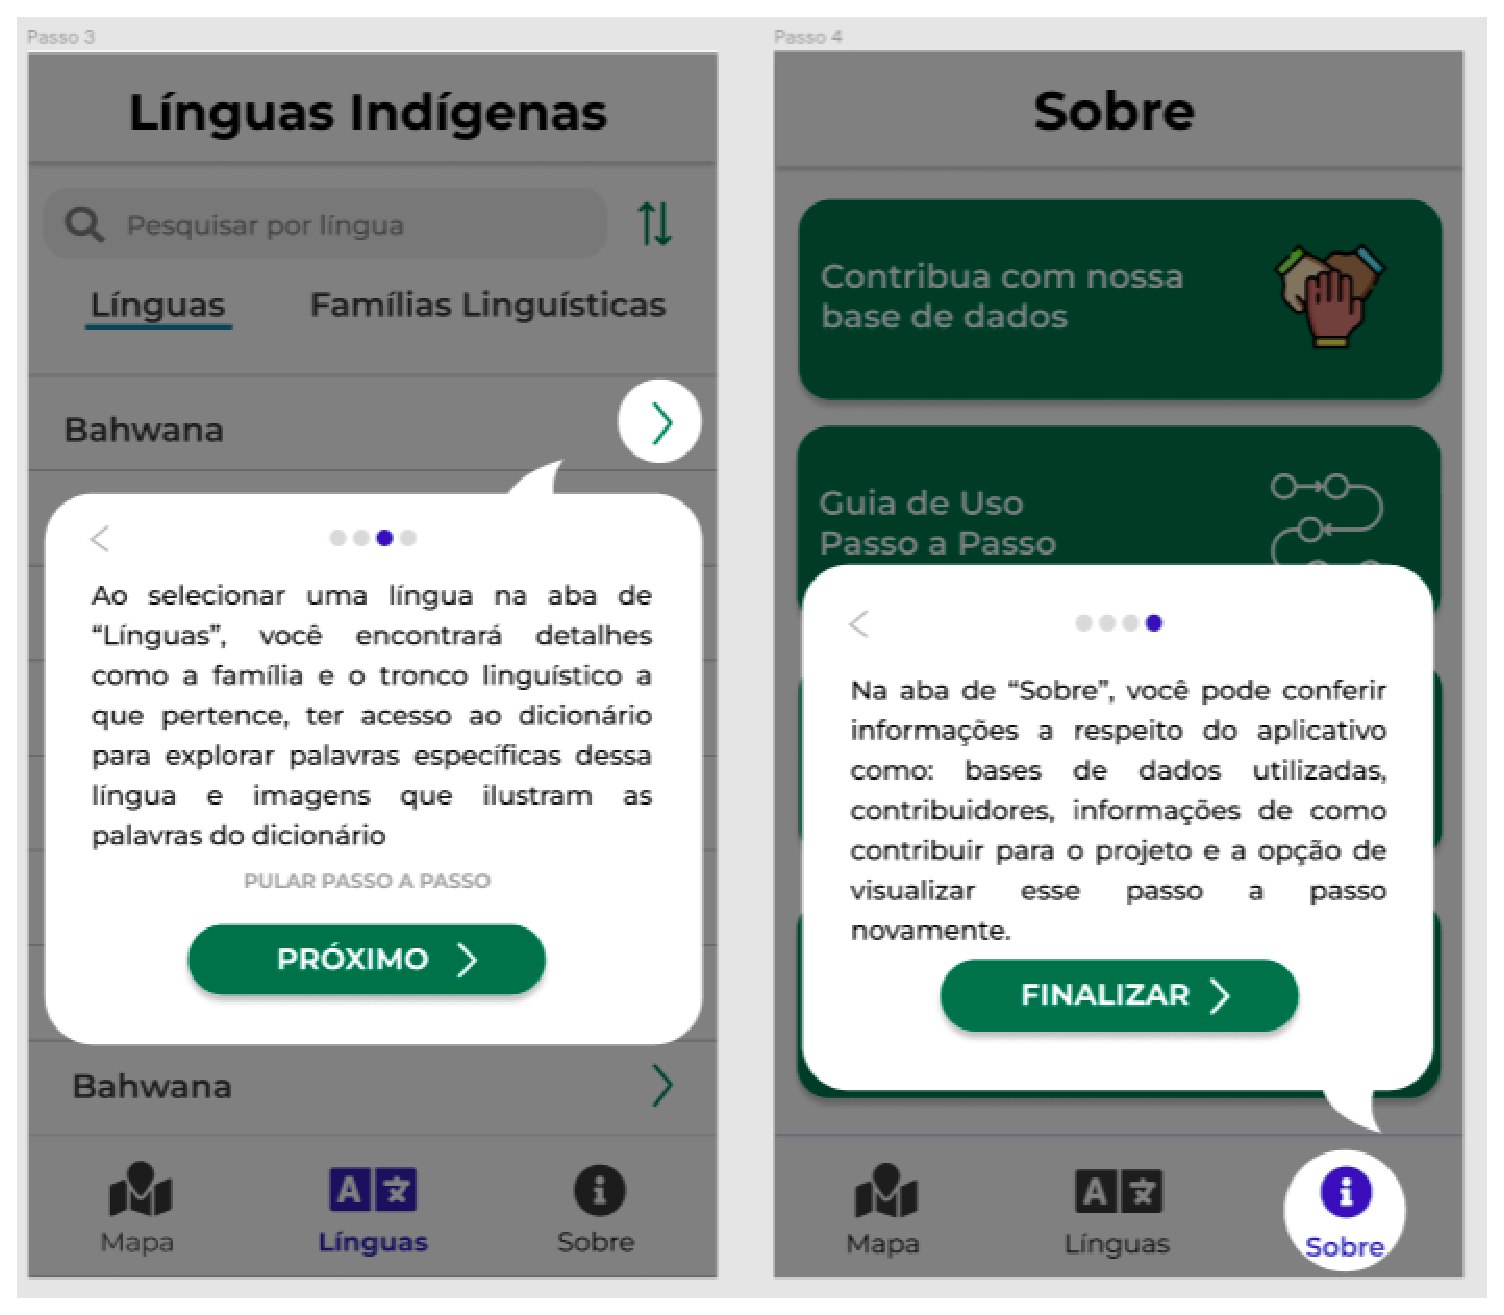
\includegraphics[width=0.8\textwidth]{figuras/onboarding1.eps}
	\end{adjustbox}
	\begin{tablenotes}[flushleft]
		\centering
		\item \textit{Fonte:} Autora.
	\end{tablenotes}
	\label{fig23}
\end{figure}

A implementação de \textit{onboarding} colabora com algumas heurísticas, como "Ajuda e Documentação", apresentando instruções claras e orientações que ajudam os usuários a entender como usar a aplicação, 
"Visibilidade do \textit{status} do sistema'', pois em cada passo apresentado é possível visualizar indicador de progresso, ou seja, o usuário possui clareza de onde está e quantos passos restantes possui. 
É possível destacar, ainda, a "Correspondência entre o sistema e o mundo real'', utilizando termos e elementos com os quais os usuários possuem familiaridade, facilitando o processo de integração. Em 
relação ao "Controle e liberdade do usuário'', opções para avançar, voltar e pular o processo são fornecidas. Além disso, "Consistência e padrões'' foram seguidos, utilizando componentes reutilizáveis e 
garantindo a consistência. Por fim, a "Prevenção de erros'', por incluir dicas e exemplos visuais para orientar os usuários e  minimizar a probabilidade de cometerem erros.

\subsection{Línguas por Família Linguística}
\label{sec:Familia Linguistica}
Outro problema de usabilidade identificado foi a dificuldade dos usuários em encontrar a opção de listar por família linguística. Visto que representa uma informação importante a respeito das línguas indígenas, 
o ícone de filtro foi substituído por texto descritivo, a fim de deixar a funcionalidade mais clara e  explícita. A Figura \ref{fig24} evidencia a mudança.

\begin{figure}[h!]
	\centering
	\caption{Línguas por Família Linguística}
	\begin{adjustbox}{center}
		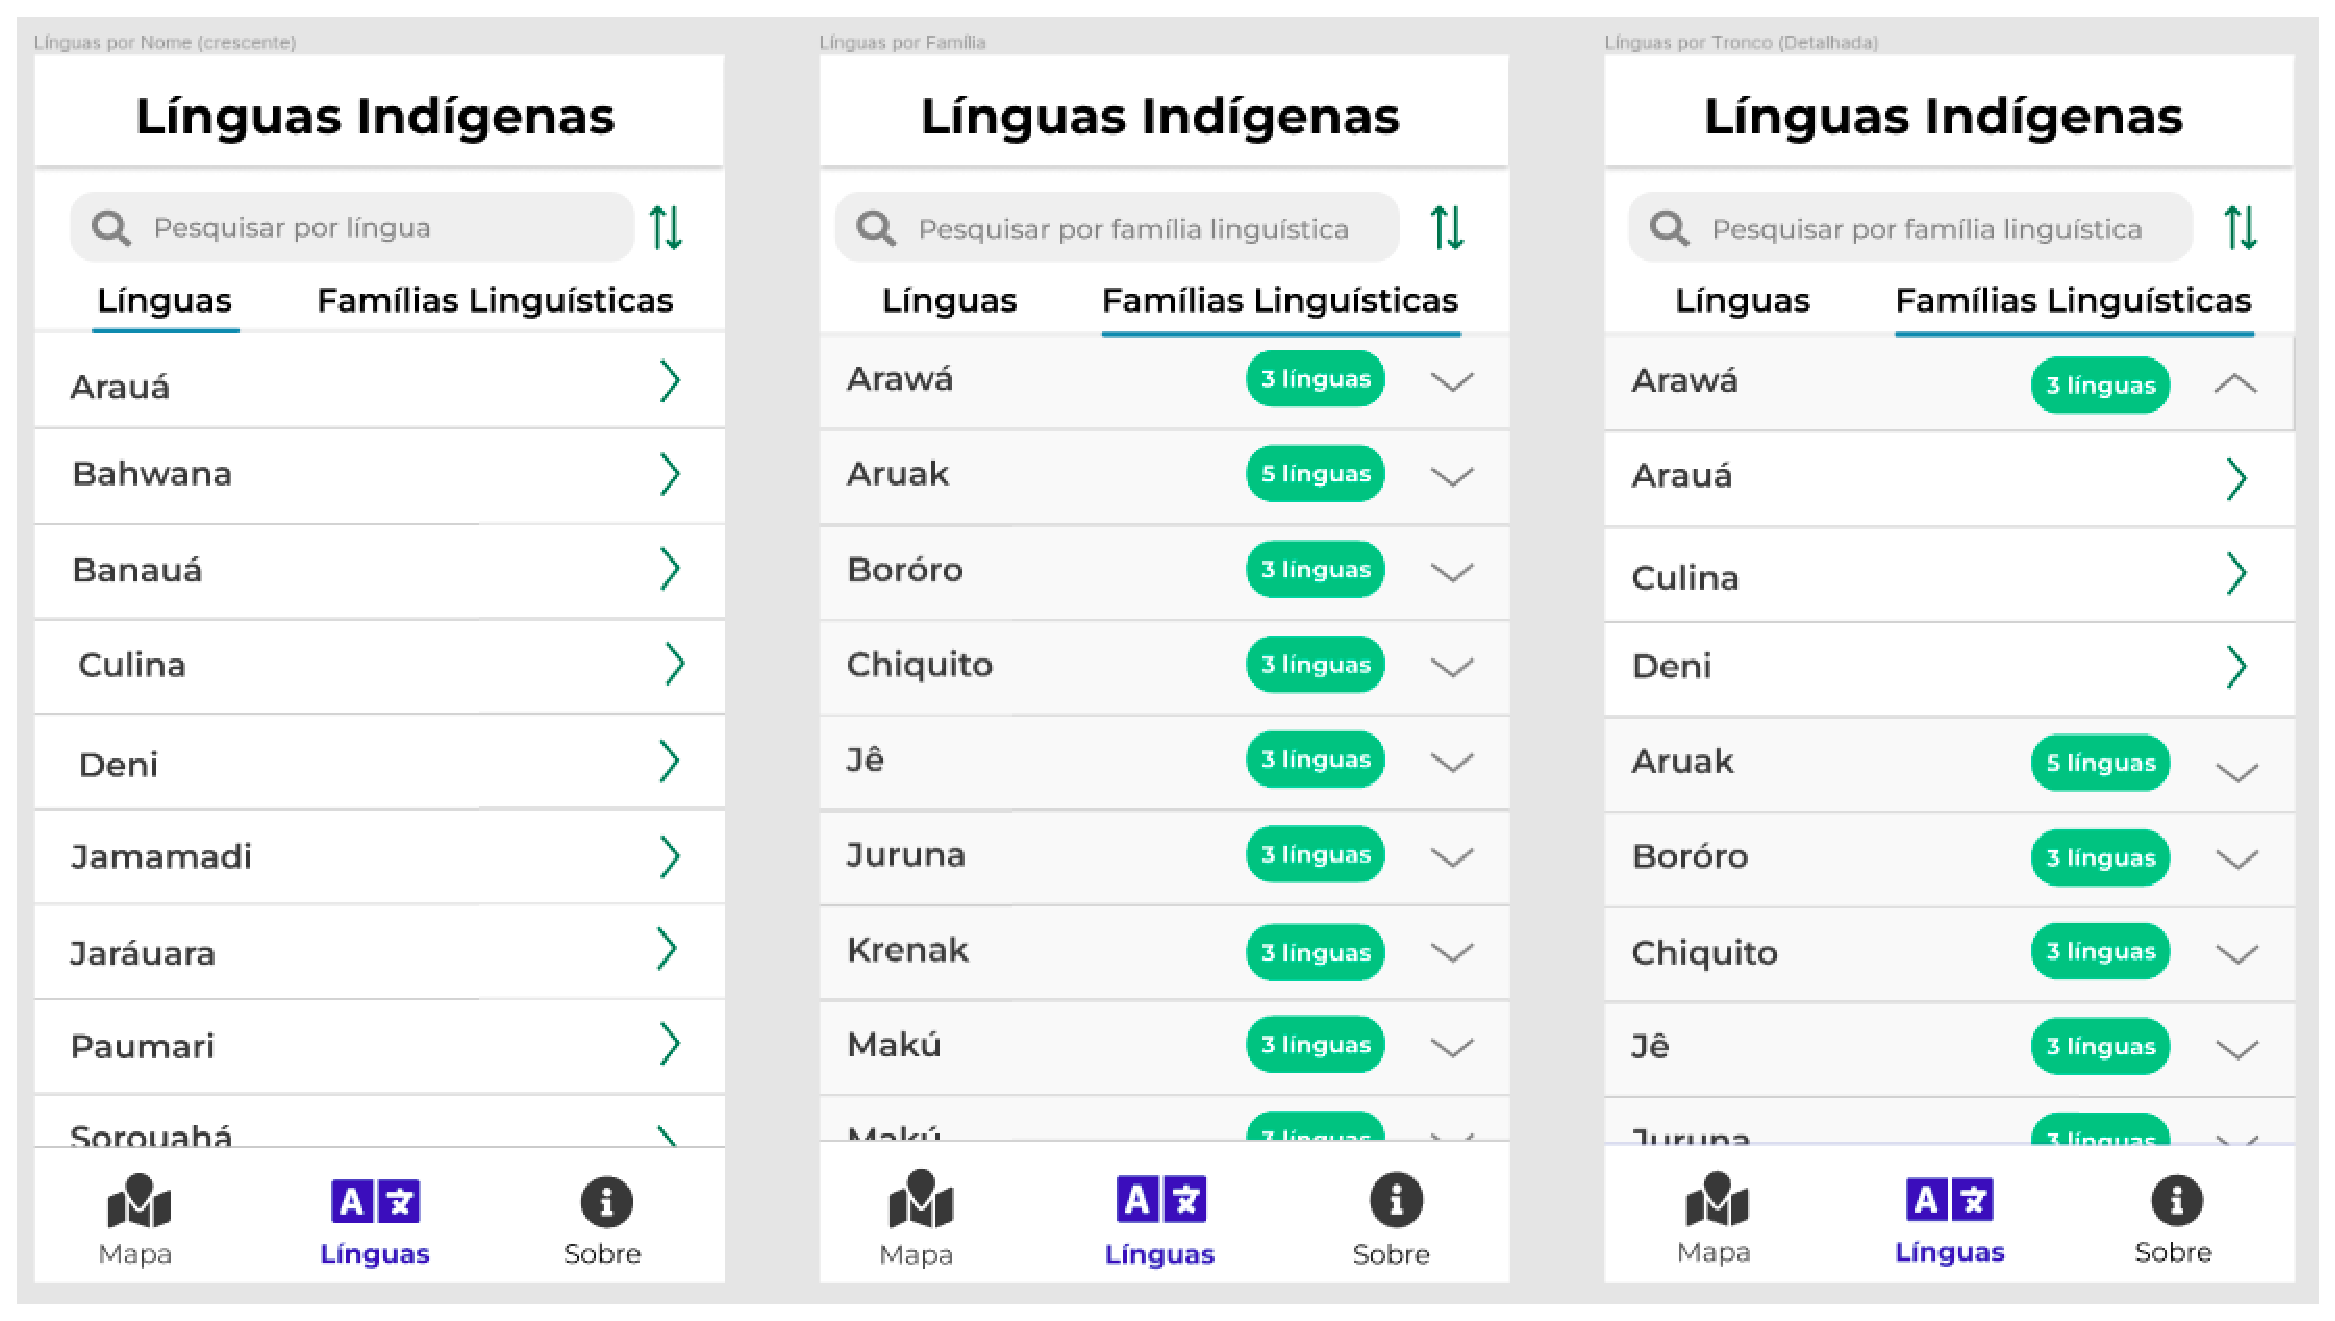
\includegraphics[width=1\textwidth]{figuras/linguas.eps}
	\end{adjustbox}
		\begin{tablenotes}[flushleft]
		\centering
		\item \textit{Fonte:} Autora.
	\end{tablenotes}
	\label{fig24}
\end{figure}

A implementação dessa troca aborda, principalmente, a heurística de "Visibilidade do \textit{status} do sistema'', pois ao substituir o ícone por um texto descritivo, os usuários terão uma compreensão mais clara e explícita da 
funcionalidade disponível, além de poderem visualizar exatamente onde estão através do componente de abas. Em relação à "Correspondência entre o sistema e o mundo real'', pode-se pontuar que a funcionalidade se torna mais 
alinhada com a expectativa do usuário. Isso ocorre, pois através do texto descritivo, os usuários podem associar mais facilmente à ação. Além disso, foi adotado o princípio de "Consistência e Padrões'', seguindo a utilização de componentes 
reutilizáveis e garantindo a coerência em todo o sistema. 

\subsection{Disposição de Informações}
\label{sec:Disposicao de Informacoes}

Entre as melhorias implementadas no aplicativo, tem-se a reorganização e a disposição das informações. A utilização de abas em diferentes telas, como as de línguas, palavras específicas e dicionário foram 
visualmente destacadas quando selecionadas, com o uso de cores distintas para indicar ao usuário em qual seção ele está navegando, conforme apresentado na Figura \ref{fig25}. Essa mudança proporciona maior visibilidade ao \textit{status} atual do sistema, tornando mais 
claro para os usuários onde eles estão e qual ação estão realizando.

\begin{figure}[h!]
	\centering
	\caption{Telas da Aplicação - Abas}
	\begin{adjustbox}{center}
		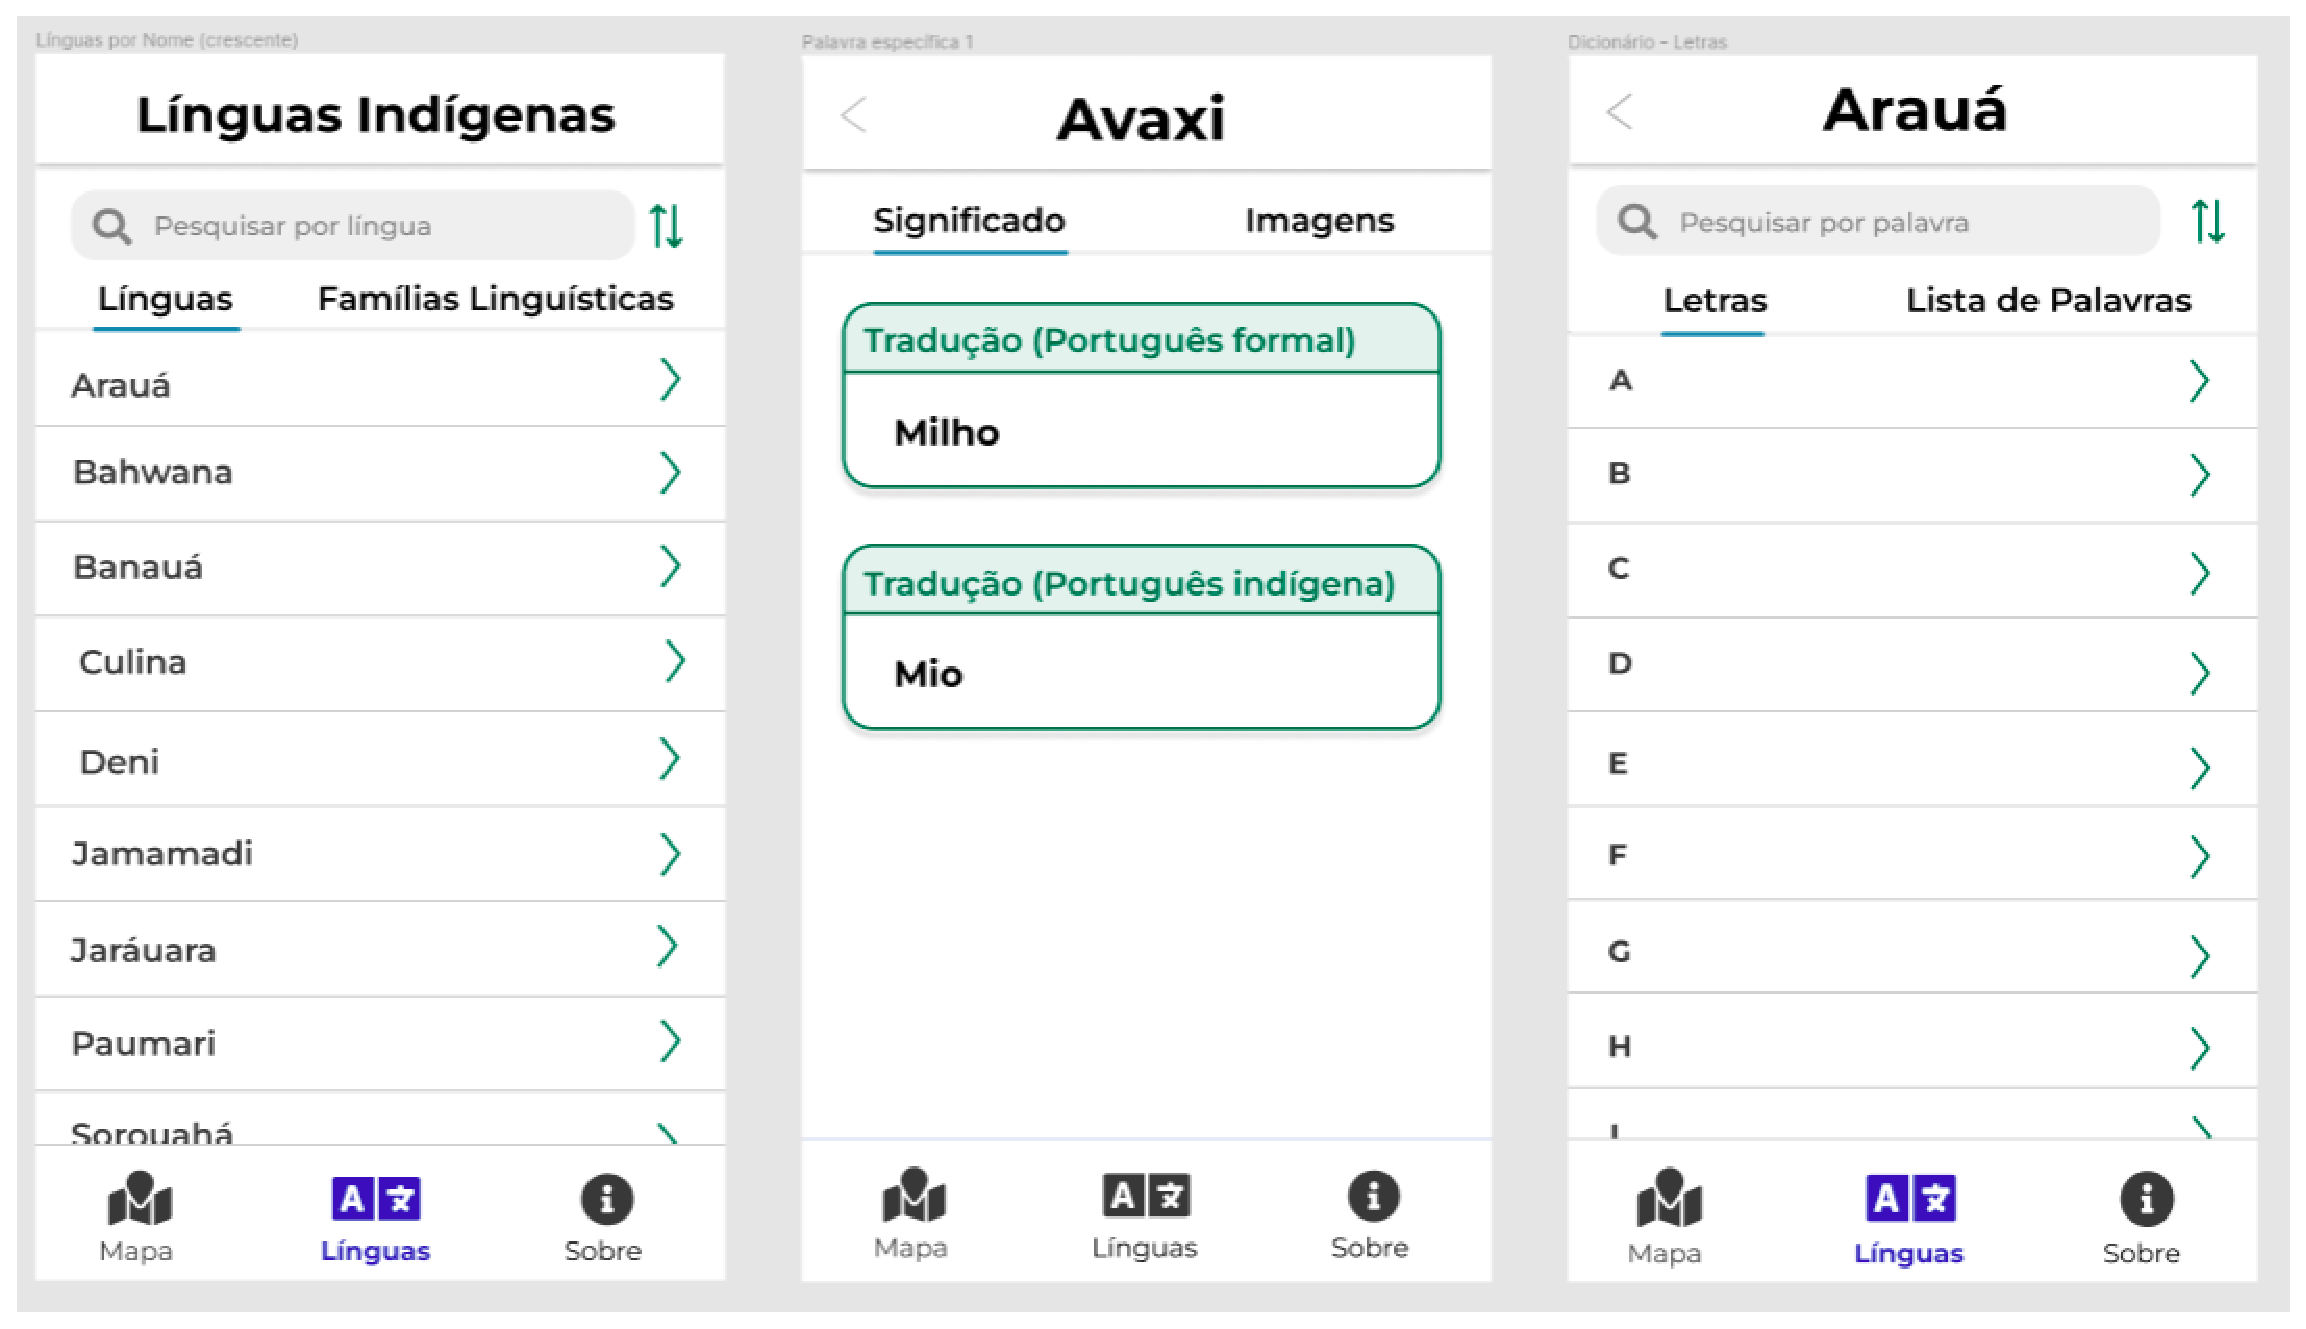
\includegraphics[width=1\textwidth]{figuras/abas.eps}
	\end{adjustbox}
	\begin{tablenotes}[flushleft]
		\centering
		\item \textit{Fonte:} Autora.
	\end{tablenotes}
	\label{fig25}
\end{figure}

Adicionalmente, visando tornar o aplicativo mais atrativo, foram adicionadas novas cores seguindo as paleta de cores da aplicação. Conforme mostra a Figura \ref{fig26}, também foram incorporados novos componentes com o objetivo de preservar a uniformidade na estrutura do aplicativo.
Essas tonalidades foram aplicadas de forma consistente no aplicativo, contribuindo para uma experiência visual mais atraente. A abordagem de "Estética e Design Minimalista'' foi adotada, evitando sobrecarregar os usuários com informações supérfluas, focando apenas no essencial.

Outra melhoria importante foi a adição da opção de contribuir com o aplicativo na tela de "Sobre", conforme ilustrado na Figura \ref{fig27}. Essa inclusão permite que os usuários tenham conhecimento sobre como podem participar ativamente do desenvolvimento do aplicativo, 
fornecendo \textit{feedback}, relatando erros e contribuindo com sugestões. Tal melhoria permite maior "Liberdade e Controle do Usuário'' na aplicação, permitindo que eles participem ativamente no desenvolvimento e aprimoramento 
das informações presentes.

Por fim, também foi definido de forma mais clara e explícita o que é o português indígena, como pode ser visto na Figura \ref{fig27}, fornecendo uma definição compreensível aos usuários. Essa informação provê uma forma de "Ajuda e Documentação'' aos usuários, promovendo uma melhor 
compreensão e orientação durante o uso do aplicativo.

\begin{figure}[h!]
	\centering
	\caption{Componentes da Aplicação}
	\begin{adjustbox}{center}
		\includegraphics[width=0.85\textwidth]{figuras/componentes.eps}
	\end{adjustbox}
	\begin{tablenotes}[flushleft]
		\centering
		\item \textit{Fonte:} Autora.
	\end{tablenotes}
	\label{fig26}
\end{figure}

\begin{figure}[h!]
	\centering
	\caption{Melhorias na disposição de informações}
	\begin{adjustbox}{center}
		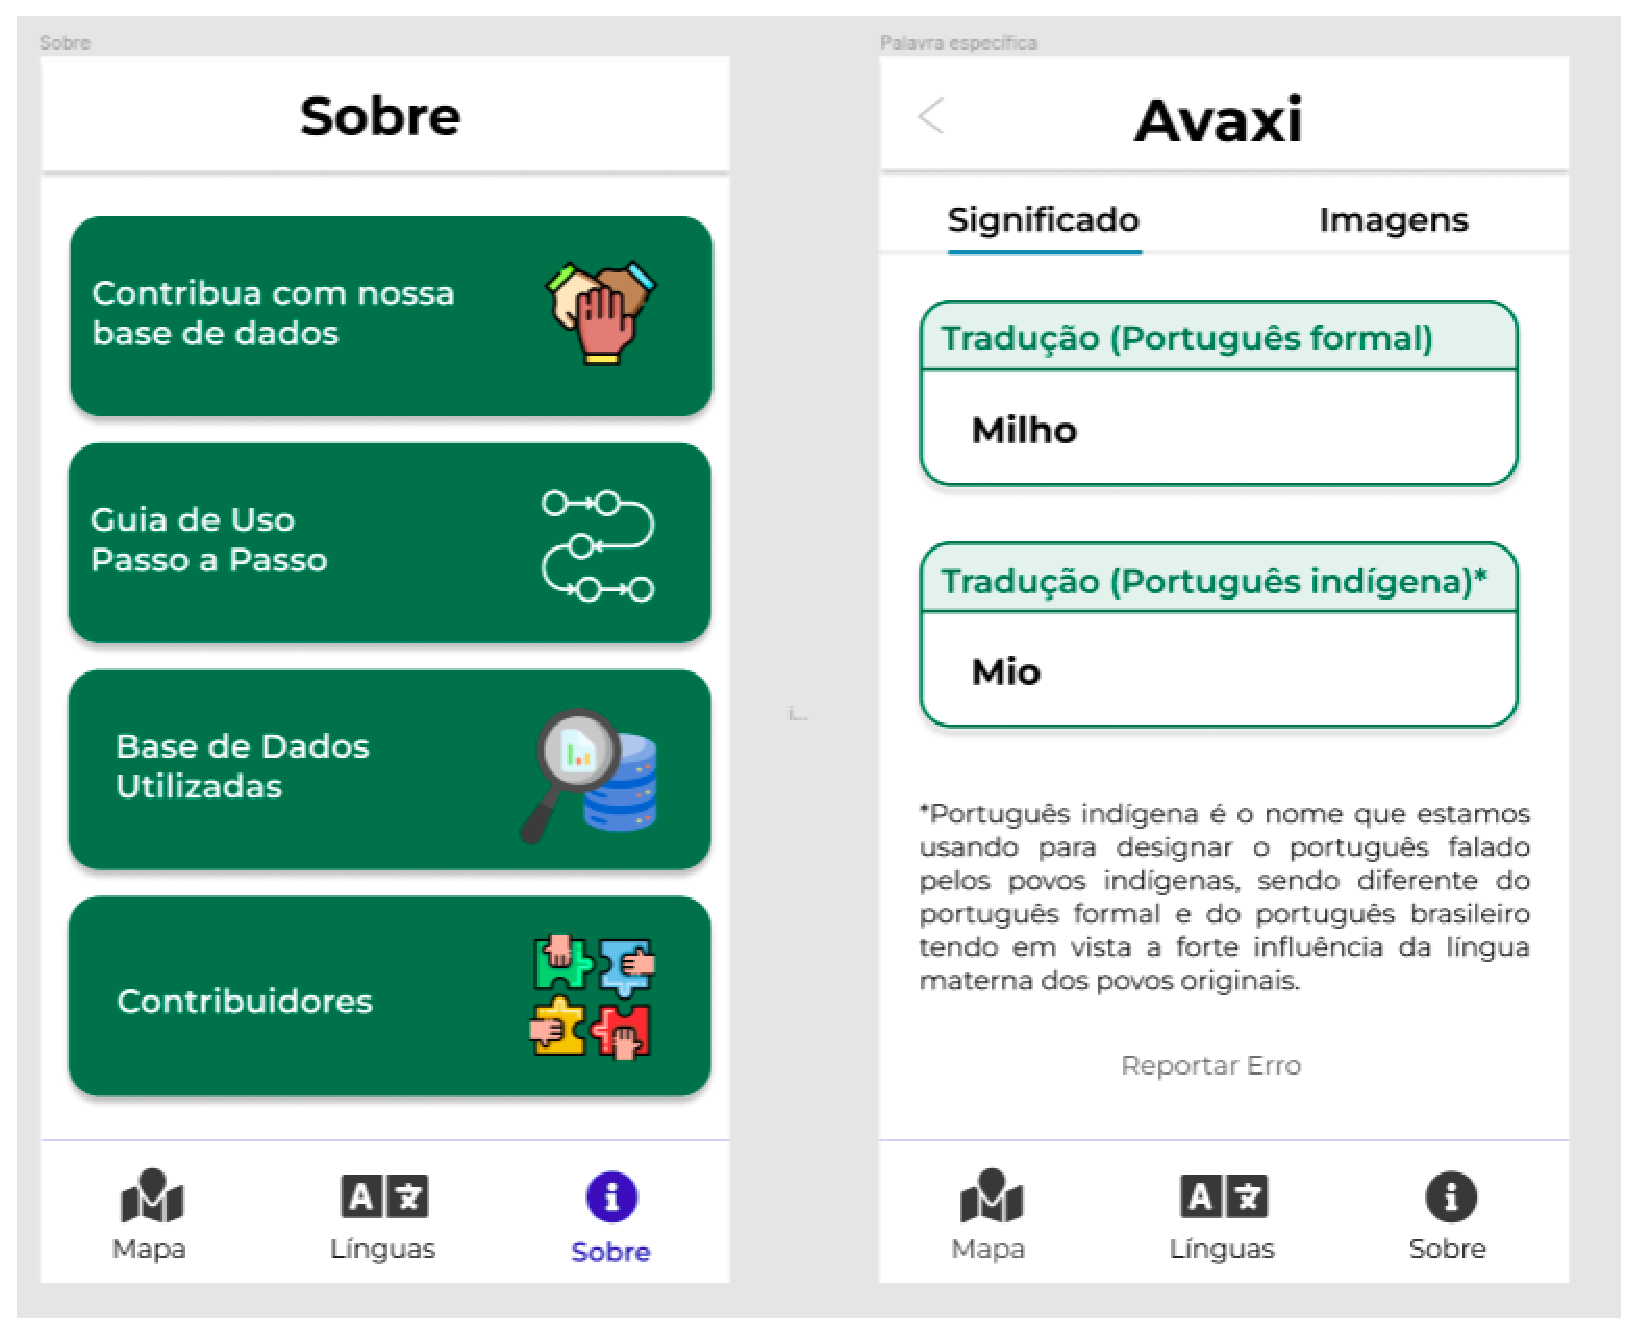
\includegraphics[width=0.7\textwidth]{figuras/melhorias.eps}
	\end{adjustbox}
	\begin{tablenotes}[flushleft]
		\centering
		\item \textit{Fonte:} Autora.
	\end{tablenotes}
	\label{fig27}
\end{figure}

\section{Matriz SWOT}
\label{sec:Matriz SWOT}

Como mencionada no \hyperref[chap:Referencial]{Capítulo 2}, a matriz SWOT oferece uma visão abrangente do aplicativo. Permitindo identificar os pontos fortes que devem ser mantidos e fortalecidos, as fraquezas que precisam ser corrigidas, as oportunidades que devem ser exploradas 
e as ameaças que devem ser enfrentadas. Essa análise é valiosa para orientar as decisões estratégicas, direcionar esforços e recursos para áreas prioritárias e identificar possíveis caminhos de desenvolvimento e aprimoramento.

No caso do aplicativo Multilind, a matriz SWOT (Figura \ref{fig30}) permitiu documentar os aspectos positivos que foram percebidos pelos usuários: as melhorias implementadas que foram bem-sucedidas (forças); as oportunidades de melhorias no aplicativo, como a introdução de funcionalidades de 
pronúncia de palavras e a ampliação da participação dos falantes das línguas indígenas (oportunidades); as áreas que ainda precisam de aprimoramento, como a necessidade de maior participação coletiva e a falta da funcionalidade de pronúncia de palavras (fraquezas), e as dificuldades 
relacionadas à tradução para o português indígena (ameaças).

\begin{figure}[h!]
	\centering
	\caption{Matriz SWOT Multilind}
	\begin{adjustbox}{center}
		\includegraphics[width=1.2\textwidth]{figuras/swot.eps}
	\end{adjustbox}
	\begin{tablenotes}[flushleft]
		\centering
		\item \textit{Fonte:} Autora.
	\end{tablenotes}
	\label{fig30}
\end{figure}



\section{Backlog de Melhorias}
\label{sec:Backlog de Melhorias}
O \textit{Product Backlog}, contendo as histórias de usuário para orientar o desenvolvimento do projeto na segunda etapa do TCC, pode ser visualizado na Tabela \ref{tab08}. Essas histórias foram elaboradas a 
partir da concepção do protótipo e das melhorias identificadas durante a pesquisa.. Além disso, a técnica MoSCoW foi utilizada para realizar a priorização. Seguindo essa classificação, os requisitos são 
categorizados como \textit{Must Have}, \textit{Should Have}, \textit{Could Have} e \textit{Won't Have} \cite{miranda2021}, na ordem dos mais necessários aos que não fazem parte do escopo. No caso, foram 
classificados em \textit{Must Have (Must)} e \textit{Should Have (Should)}, conferindo ênfase ao que de fato faz parte do escopo de implementação desse projeto.

\begin{table}[h!]
	\centering
	\caption{\textit{Backlog}}
	\label{tab08}
	\begin{tabularx}{\textwidth}{p{1cm}|p{12cm}|p{1cm}}
	\hline
	ID   & História de Usuário                                                                                                                                                                                                   & Priorização \\ \hline
	US01 & Eu, como usuário, desejo ter um processo de \textit{onboarding} no aplicativo que me guie de forma clara e intuitiva pelas funcionalidades e navegação disponíveis.                                                            & \textit{Must}        \\
	US02 & Eu, como usuário, desejo visualizar línguas por família linguística por meio de abas na tela de Línguas                                                                                                               & \textit{Must}        \\
	US03 & Eu, como usuário, desejo ter a opção de trocar de abas em vez de mudar de página para visualizar imagens e traduções relativas a uma palavra específica, facilitando o acesso.                                        & \textit{Must}        \\
	US04 & Eu, como usuário, desejo ter uma forma fácil e acessível de obter informações sobre como posso contribuir para a base de dados do aplicativo.                                                                         & \textit{Must}        \\
	US05 & Eu, como usuário, desejo ter acesso direto à lista de palavras no dicionário, para facilitar a navegação e pesquisa.																									 & \textit{Must}        \\
	US06 & Eu, como usuário, desejo obter uma explicação clara sobre o que é o português indígena, a fim de compreender melhor sua definição e significado.                                                                      & \textit{Must}        \\
	US07 & Eu, como usuário, desejo que o design da aplicação seja mais atraente e visualmente agradável, através da adição de mais cores que complementem a interface.                                                          & \textit{Should}      \\
	US08 & Eu, como usuário, desejo obter informações precisas sobre o nome da língua do português indígena que está relacionada a uma língua específica, a fim de compreender melhor sua classificação linguística. 			 & \textit{Should}      \\
	US09 & Eu, como usuário, desejo ter a opção de relatar erros ou inconsistências nas traduções e imagens das palavras, a fim de contribuir para a consistência das informações apresentadas.                                  & \textit{Should}      \\
	US10 & Eu, como usuário, desejo ter a opção de ouvir a pronúncia correta das palavras no aplicativo, a fim de melhorar minha compreensão e pronúncia adequada.                                                               & \textit{Should}      \\ \hline
	\end{tabularx}
\end{table}

\section{Desenvolvimento do Aplicativo}
\label{sec:Desenvolvimento do Aplicativo}

\section{Resumo do Capítulo}
\label{sec:Resumo Proposta}
No capítulo em questão, o contexto no qual o trabalho se propõe a contribuir é revisado, e a proposta do Trabalho de Conclusão de Curso é apresentada. A seção de \hyperref[sec:Contextualização]{Contextualização} fornece informações sobre o domínio no qual o estudo está inserido. Além disso, 
a seção de \hyperref[sec:Detalhamento da Aplicacao]{Detalhamento da Aplicação} é apresentada para garantir uma adequada compreensão da aplicação Multilind. Além disso, a seção de \hyperref[sec:Backlog de Melhorias]{\textit{Backlog} de Melhorias} apresenta uma lista priorizada das funcionalidades que serão implementadas na próxima etapa desse TCC. 
